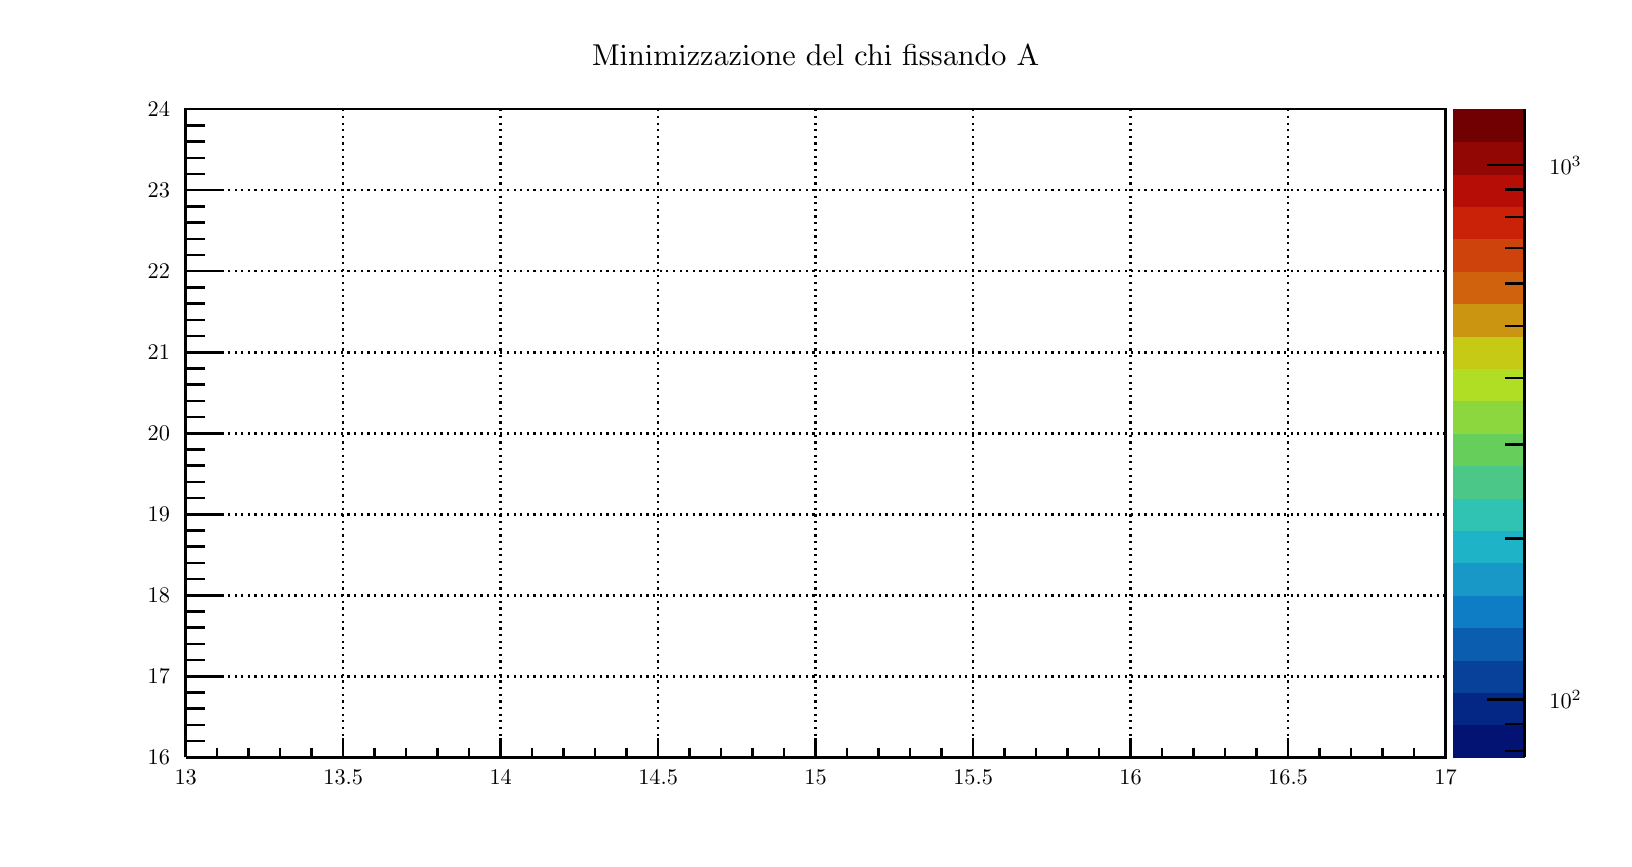
\begin{tikzpicture}
\pgfdeclareplotmark{cross} {
\pgfpathmoveto{\pgfpoint{-0.3\pgfplotmarksize}{\pgfplotmarksize}}
\pgfpathlineto{\pgfpoint{+0.3\pgfplotmarksize}{\pgfplotmarksize}}
\pgfpathlineto{\pgfpoint{+0.3\pgfplotmarksize}{0.3\pgfplotmarksize}}
\pgfpathlineto{\pgfpoint{+1\pgfplotmarksize}{0.3\pgfplotmarksize}}
\pgfpathlineto{\pgfpoint{+1\pgfplotmarksize}{-0.3\pgfplotmarksize}}
\pgfpathlineto{\pgfpoint{+0.3\pgfplotmarksize}{-0.3\pgfplotmarksize}}
\pgfpathlineto{\pgfpoint{+0.3\pgfplotmarksize}{-1.\pgfplotmarksize}}
\pgfpathlineto{\pgfpoint{-0.3\pgfplotmarksize}{-1.\pgfplotmarksize}}
\pgfpathlineto{\pgfpoint{-0.3\pgfplotmarksize}{-0.3\pgfplotmarksize}}
\pgfpathlineto{\pgfpoint{-1.\pgfplotmarksize}{-0.3\pgfplotmarksize}}
\pgfpathlineto{\pgfpoint{-1.\pgfplotmarksize}{0.3\pgfplotmarksize}}
\pgfpathlineto{\pgfpoint{-0.3\pgfplotmarksize}{0.3\pgfplotmarksize}}
\pgfpathclose
\pgfusepathqstroke
}
\pgfdeclareplotmark{cross*} {
\pgfpathmoveto{\pgfpoint{-0.3\pgfplotmarksize}{\pgfplotmarksize}}
\pgfpathlineto{\pgfpoint{+0.3\pgfplotmarksize}{\pgfplotmarksize}}
\pgfpathlineto{\pgfpoint{+0.3\pgfplotmarksize}{0.3\pgfplotmarksize}}
\pgfpathlineto{\pgfpoint{+1\pgfplotmarksize}{0.3\pgfplotmarksize}}
\pgfpathlineto{\pgfpoint{+1\pgfplotmarksize}{-0.3\pgfplotmarksize}}
\pgfpathlineto{\pgfpoint{+0.3\pgfplotmarksize}{-0.3\pgfplotmarksize}}
\pgfpathlineto{\pgfpoint{+0.3\pgfplotmarksize}{-1.\pgfplotmarksize}}
\pgfpathlineto{\pgfpoint{-0.3\pgfplotmarksize}{-1.\pgfplotmarksize}}
\pgfpathlineto{\pgfpoint{-0.3\pgfplotmarksize}{-0.3\pgfplotmarksize}}
\pgfpathlineto{\pgfpoint{-1.\pgfplotmarksize}{-0.3\pgfplotmarksize}}
\pgfpathlineto{\pgfpoint{-1.\pgfplotmarksize}{0.3\pgfplotmarksize}}
\pgfpathlineto{\pgfpoint{-0.3\pgfplotmarksize}{0.3\pgfplotmarksize}}
\pgfpathclose
\pgfusepathqfillstroke
}
\pgfdeclareplotmark{newstar} {
\pgfpathmoveto{\pgfqpoint{0pt}{\pgfplotmarksize}}
\pgfpathlineto{\pgfqpointpolar{44}{0.5\pgfplotmarksize}}
\pgfpathlineto{\pgfqpointpolar{18}{\pgfplotmarksize}}
\pgfpathlineto{\pgfqpointpolar{-20}{0.5\pgfplotmarksize}}
\pgfpathlineto{\pgfqpointpolar{-54}{\pgfplotmarksize}}
\pgfpathlineto{\pgfqpointpolar{-90}{0.5\pgfplotmarksize}}
\pgfpathlineto{\pgfqpointpolar{234}{\pgfplotmarksize}}
\pgfpathlineto{\pgfqpointpolar{198}{0.5\pgfplotmarksize}}
\pgfpathlineto{\pgfqpointpolar{162}{\pgfplotmarksize}}
\pgfpathlineto{\pgfqpointpolar{134}{0.5\pgfplotmarksize}}
\pgfpathclose
\pgfusepathqstroke
}
\pgfdeclareplotmark{newstar*} {
\pgfpathmoveto{\pgfqpoint{0pt}{\pgfplotmarksize}}
\pgfpathlineto{\pgfqpointpolar{44}{0.5\pgfplotmarksize}}
\pgfpathlineto{\pgfqpointpolar{18}{\pgfplotmarksize}}
\pgfpathlineto{\pgfqpointpolar{-20}{0.5\pgfplotmarksize}}
\pgfpathlineto{\pgfqpointpolar{-54}{\pgfplotmarksize}}
\pgfpathlineto{\pgfqpointpolar{-90}{0.5\pgfplotmarksize}}
\pgfpathlineto{\pgfqpointpolar{234}{\pgfplotmarksize}}
\pgfpathlineto{\pgfqpointpolar{198}{0.5\pgfplotmarksize}}
\pgfpathlineto{\pgfqpointpolar{162}{\pgfplotmarksize}}
\pgfpathlineto{\pgfqpointpolar{134}{0.5\pgfplotmarksize}}
\pgfpathclose
\pgfusepathqfillstroke
}
\definecolor{c}{rgb}{1,1,1};
\draw [color=c, fill=c] (0,0) rectangle (20,10.2882);
\draw [color=c, fill=c] (2,1.02882) rectangle (18,9.25934);
\definecolor{c}{rgb}{0,0,0};
\draw [c,line width=0.9] (2,1.02882) -- (2,9.25934) -- (18,9.25934) -- (18,1.02882) -- (2,1.02882);
\definecolor{c}{rgb}{1,1,1};
\draw [color=c, fill=c] (2,1.02882) rectangle (18,9.25934);
\definecolor{c}{rgb}{0,0,0};
\draw [c,line width=0.9] (2,1.02882) -- (2,9.25934) -- (18,9.25934) -- (18,1.02882) -- (2,1.02882);
\draw [c,line width=0.9] (2,1.02882) -- (18,1.02882);
\draw [c,line width=0.9] (2,1.27573) -- (2,1.02882);
\draw [c,dash pattern=on 0.80pt off 1.60pt ,line width=0.9] (2,9.25934) -- (2,1.02882);
\draw [c,line width=0.9] (2.4,1.15227) -- (2.4,1.02882);
\draw [c,line width=0.9] (2.8,1.15227) -- (2.8,1.02882);
\draw [c,line width=0.9] (3.2,1.15227) -- (3.2,1.02882);
\draw [c,line width=0.9] (3.6,1.15227) -- (3.6,1.02882);
\draw [c,line width=0.9] (4,1.27573) -- (4,1.02882);
\draw [c,dash pattern=on 0.80pt off 1.60pt ,line width=0.9] (4,9.25934) -- (4,1.02882);
\draw [c,line width=0.9] (4.4,1.15227) -- (4.4,1.02882);
\draw [c,line width=0.9] (4.8,1.15227) -- (4.8,1.02882);
\draw [c,line width=0.9] (5.2,1.15227) -- (5.2,1.02882);
\draw [c,line width=0.9] (5.6,1.15227) -- (5.6,1.02882);
\draw [c,line width=0.9] (6,1.27573) -- (6,1.02882);
\draw [c,dash pattern=on 0.80pt off 1.60pt ,line width=0.9] (6,9.25934) -- (6,1.02882);
\draw [c,line width=0.9] (6.4,1.15227) -- (6.4,1.02882);
\draw [c,line width=0.9] (6.8,1.15227) -- (6.8,1.02882);
\draw [c,line width=0.9] (7.2,1.15227) -- (7.2,1.02882);
\draw [c,line width=0.9] (7.6,1.15227) -- (7.6,1.02882);
\draw [c,line width=0.9] (8,1.27573) -- (8,1.02882);
\draw [c,dash pattern=on 0.80pt off 1.60pt ,line width=0.9] (8,9.25934) -- (8,1.02882);
\draw [c,line width=0.9] (8.4,1.15227) -- (8.4,1.02882);
\draw [c,line width=0.9] (8.8,1.15227) -- (8.8,1.02882);
\draw [c,line width=0.9] (9.2,1.15227) -- (9.2,1.02882);
\draw [c,line width=0.9] (9.6,1.15227) -- (9.6,1.02882);
\draw [c,line width=0.9] (10,1.27573) -- (10,1.02882);
\draw [c,dash pattern=on 0.80pt off 1.60pt ,line width=0.9] (10,9.25934) -- (10,1.02882);
\draw [c,line width=0.9] (10.4,1.15227) -- (10.4,1.02882);
\draw [c,line width=0.9] (10.8,1.15227) -- (10.8,1.02882);
\draw [c,line width=0.9] (11.2,1.15227) -- (11.2,1.02882);
\draw [c,line width=0.9] (11.6,1.15227) -- (11.6,1.02882);
\draw [c,line width=0.9] (12,1.27573) -- (12,1.02882);
\draw [c,dash pattern=on 0.80pt off 1.60pt ,line width=0.9] (12,9.25934) -- (12,1.02882);
\draw [c,line width=0.9] (12.4,1.15227) -- (12.4,1.02882);
\draw [c,line width=0.9] (12.8,1.15227) -- (12.8,1.02882);
\draw [c,line width=0.9] (13.2,1.15227) -- (13.2,1.02882);
\draw [c,line width=0.9] (13.6,1.15227) -- (13.6,1.02882);
\draw [c,line width=0.9] (14,1.27573) -- (14,1.02882);
\draw [c,dash pattern=on 0.80pt off 1.60pt ,line width=0.9] (14,9.25934) -- (14,1.02882);
\draw [c,line width=0.9] (14.4,1.15227) -- (14.4,1.02882);
\draw [c,line width=0.9] (14.8,1.15227) -- (14.8,1.02882);
\draw [c,line width=0.9] (15.2,1.15227) -- (15.2,1.02882);
\draw [c,line width=0.9] (15.6,1.15227) -- (15.6,1.02882);
\draw [c,line width=0.9] (16,1.27573) -- (16,1.02882);
\draw [c,dash pattern=on 0.80pt off 1.60pt ,line width=0.9] (16,9.25934) -- (16,1.02882);
\draw [c,line width=0.9] (16.4,1.15227) -- (16.4,1.02882);
\draw [c,line width=0.9] (16.8,1.15227) -- (16.8,1.02882);
\draw [c,line width=0.9] (17.2,1.15227) -- (17.2,1.02882);
\draw [c,line width=0.9] (17.6,1.15227) -- (17.6,1.02882);
\draw [c,line width=0.9] (18,1.27573) -- (18,1.02882);
\draw [c,dash pattern=on 0.80pt off 1.60pt ,line width=0.9] (18,9.25934) -- (18,1.02882);
\draw [anchor=base] (2,0.689306) node[scale=0.805902, color=c, rotate=0]{13};
\draw [anchor=base] (4,0.689306) node[scale=0.805902, color=c, rotate=0]{13.5};
\draw [anchor=base] (6,0.689306) node[scale=0.805902, color=c, rotate=0]{14};
\draw [anchor=base] (8,0.689306) node[scale=0.805902, color=c, rotate=0]{14.5};
\draw [anchor=base] (10,0.689306) node[scale=0.805902, color=c, rotate=0]{15};
\draw [anchor=base] (12,0.689306) node[scale=0.805902, color=c, rotate=0]{15.5};
\draw [anchor=base] (14,0.689306) node[scale=0.805902, color=c, rotate=0]{16};
\draw [anchor=base] (16,0.689306) node[scale=0.805902, color=c, rotate=0]{16.5};
\draw [anchor=base] (18,0.689306) node[scale=0.805902, color=c, rotate=0]{17};
\draw [c,line width=0.9] (2,1.02882) -- (2,9.25934);
\draw [c,line width=0.9] (2.48,1.02882) -- (2,1.02882);
\draw [c,dash pattern=on 0.80pt off 1.60pt ,line width=0.9] (18,1.02882) -- (2,1.02882);
\draw [c,line width=0.9] (2.24,1.23458) -- (2,1.23458);
\draw [c,line width=0.9] (2.24,1.44034) -- (2,1.44034);
\draw [c,line width=0.9] (2.24,1.6461) -- (2,1.6461);
\draw [c,line width=0.9] (2.24,1.85187) -- (2,1.85187);
\draw [c,line width=0.9] (2.48,2.05763) -- (2,2.05763);
\draw [c,dash pattern=on 0.80pt off 1.60pt ,line width=0.9] (18,2.05763) -- (2,2.05763);
\draw [c,line width=0.9] (2.24,2.26339) -- (2,2.26339);
\draw [c,line width=0.9] (2.24,2.46916) -- (2,2.46916);
\draw [c,line width=0.9] (2.24,2.67492) -- (2,2.67492);
\draw [c,line width=0.9] (2.24,2.88068) -- (2,2.88068);
\draw [c,line width=0.9] (2.48,3.08645) -- (2,3.08645);
\draw [c,dash pattern=on 0.80pt off 1.60pt ,line width=0.9] (18,3.08645) -- (2,3.08645);
\draw [c,line width=0.9] (2.24,3.29221) -- (2,3.29221);
\draw [c,line width=0.9] (2.24,3.49797) -- (2,3.49797);
\draw [c,line width=0.9] (2.24,3.70374) -- (2,3.70374);
\draw [c,line width=0.9] (2.24,3.9095) -- (2,3.9095);
\draw [c,line width=0.9] (2.48,4.11526) -- (2,4.11526);
\draw [c,dash pattern=on 0.80pt off 1.60pt ,line width=0.9] (18,4.11526) -- (2,4.11526);
\draw [c,line width=0.9] (2.24,4.32102) -- (2,4.32102);
\draw [c,line width=0.9] (2.24,4.52679) -- (2,4.52679);
\draw [c,line width=0.9] (2.24,4.73255) -- (2,4.73255);
\draw [c,line width=0.9] (2.24,4.93831) -- (2,4.93831);
\draw [c,line width=0.9] (2.48,5.14408) -- (2,5.14408);
\draw [c,dash pattern=on 0.80pt off 1.60pt ,line width=0.9] (18,5.14408) -- (2,5.14408);
\draw [c,line width=0.9] (2.24,5.34984) -- (2,5.34984);
\draw [c,line width=0.9] (2.24,5.5556) -- (2,5.5556);
\draw [c,line width=0.9] (2.24,5.76137) -- (2,5.76137);
\draw [c,line width=0.9] (2.24,5.96713) -- (2,5.96713);
\draw [c,line width=0.9] (2.48,6.17289) -- (2,6.17289);
\draw [c,dash pattern=on 0.80pt off 1.60pt ,line width=0.9] (18,6.17289) -- (2,6.17289);
\draw [c,line width=0.9] (2.24,6.37866) -- (2,6.37866);
\draw [c,line width=0.9] (2.24,6.58442) -- (2,6.58442);
\draw [c,line width=0.9] (2.24,6.79018) -- (2,6.79018);
\draw [c,line width=0.9] (2.24,6.99594) -- (2,6.99594);
\draw [c,line width=0.9] (2.48,7.20171) -- (2,7.20171);
\draw [c,dash pattern=on 0.80pt off 1.60pt ,line width=0.9] (18,7.20171) -- (2,7.20171);
\draw [c,line width=0.9] (2.24,7.40747) -- (2,7.40747);
\draw [c,line width=0.9] (2.24,7.61323) -- (2,7.61323);
\draw [c,line width=0.9] (2.24,7.819) -- (2,7.819);
\draw [c,line width=0.9] (2.24,8.02476) -- (2,8.02476);
\draw [c,line width=0.9] (2.48,8.23052) -- (2,8.23052);
\draw [c,dash pattern=on 0.80pt off 1.60pt ,line width=0.9] (18,8.23052) -- (2,8.23052);
\draw [c,line width=0.9] (2.24,8.43629) -- (2,8.43629);
\draw [c,line width=0.9] (2.24,8.64205) -- (2,8.64205);
\draw [c,line width=0.9] (2.24,8.84781) -- (2,8.84781);
\draw [c,line width=0.9] (2.24,9.05358) -- (2,9.05358);
\draw [c,line width=0.9] (2.48,9.25934) -- (2,9.25934);
\draw [c,dash pattern=on 0.80pt off 1.60pt ,line width=0.9] (18,9.25934) -- (2,9.25934);
\draw [anchor= east] (1.9,1.02882) node[scale=0.805902, color=c, rotate=0]{16};
\draw [anchor= east] (1.9,2.05763) node[scale=0.805902, color=c, rotate=0]{17};
\draw [anchor= east] (1.9,3.08645) node[scale=0.805902, color=c, rotate=0]{18};
\draw [anchor= east] (1.9,4.11526) node[scale=0.805902, color=c, rotate=0]{19};
\draw [anchor= east] (1.9,5.14408) node[scale=0.805902, color=c, rotate=0]{20};
\draw [anchor= east] (1.9,6.17289) node[scale=0.805902, color=c, rotate=0]{21};
\draw [anchor= east] (1.9,7.20171) node[scale=0.805902, color=c, rotate=0]{22};
\draw [anchor= east] (1.9,8.23052) node[scale=0.805902, color=c, rotate=0]{23};
\draw [anchor= east] (1.9,9.25934) node[scale=0.805902, color=c, rotate=0]{24};
\definecolor{c}{rgb}{0.00759013,0.0728653,0.45351};
\draw [color=c, fill=c] (18.1,1.02882) rectangle (19,1.44034);
\definecolor{c}{rgb}{0.0158128,0.151803,0.524225};
\draw [color=c, fill=c] (18.1,1.44034) rectangle (19,1.85187);
\definecolor{c}{rgb}{0.0281863,0.253431,0.604902};
\draw [color=c, fill=c] (18.1,1.85187) rectangle (19,2.26339);
\definecolor{c}{rgb}{0.0428922,0.365196,0.687255};
\draw [color=c, fill=c] (18.1,2.26339) rectangle (19,2.67492);
\definecolor{c}{rgb}{0.0588235,0.486275,0.776471};
\draw [color=c, fill=c] (18.1,2.67492) rectangle (19,3.08645);
\definecolor{c}{rgb}{0.0906863,0.594608,0.78125};
\draw [color=c, fill=c] (18.1,3.08645) rectangle (19,3.49797);
\definecolor{c}{rgb}{0.122549,0.702941,0.786029};
\draw [color=c, fill=c] (18.1,3.49797) rectangle (19,3.9095);
\definecolor{c}{rgb}{0.18652,0.763235,0.706618};
\draw [color=c, fill=c] (18.1,3.9095) rectangle (19,4.32102);
\definecolor{c}{rgb}{0.29326,0.785539,0.529779};
\draw [color=c, fill=c] (18.1,4.32102) rectangle (19,4.73255);
\definecolor{c}{rgb}{0.4,0.807843,0.352941};
\draw [color=c, fill=c] (18.1,4.73255) rectangle (19,5.14408);
\definecolor{c}{rgb}{0.549755,0.839706,0.244608};
\draw [color=c, fill=c] (18.1,5.14408) rectangle (19,5.5556);
\definecolor{c}{rgb}{0.68799,0.869118,0.144608};
\draw [color=c, fill=c] (18.1,5.5556) rectangle (19,5.96713);
\definecolor{c}{rgb}{0.777451,0.791422,0.0796569};
\draw [color=c, fill=c] (18.1,5.96713) rectangle (19,6.37866);
\definecolor{c}{rgb}{0.796569,0.585907,0.0653186};
\draw [color=c, fill=c] (18.1,6.37866) rectangle (19,6.79018);
\definecolor{c}{rgb}{0.815686,0.380392,0.0509804};
\draw [color=c, fill=c] (18.1,6.79018) rectangle (19,7.20171);
\definecolor{c}{rgb}{0.802451,0.261275,0.0436275};
\draw [color=c, fill=c] (18.1,7.20171) rectangle (19,7.61323);
\definecolor{c}{rgb}{0.788113,0.13223,0.0356618};
\draw [color=c, fill=c] (18.1,7.61323) rectangle (19,8.02476);
\definecolor{c}{rgb}{0.714951,0.0509804,0.0269608};
\draw [color=c, fill=c] (18.1,8.02476) rectangle (19,8.43629);
\definecolor{c}{rgb}{0.573162,0.0254902,0.017402};
\draw [color=c, fill=c] (18.1,8.43629) rectangle (19,8.84781);
\definecolor{c}{rgb}{0.442279,0.00196078,0.00857843};
\draw [color=c, fill=c] (18.1,8.84781) rectangle (19,9.25934);
\definecolor{c}{rgb}{0,0,0};
\draw [c,line width=0.9] (19,1.02882) -- (19,9.25934);
\draw [c,line width=0.9] (18.76,1.10664) -- (19,1.10664);
\draw [c,line width=0.9] (18.76,1.4537) -- (19,1.4537);
\draw [c,line width=0.9] (18.52,1.76416) -- (19,1.76416);
\draw [anchor= west] (19.219,1.76416) node[scale=0.805902, color=c, rotate=0]{$10^{2}$};
\draw [c,line width=0.9] (18.76,3.80659) -- (19,3.80659);
\draw [c,line width=0.9] (18.76,5.00134) -- (19,5.00134);
\draw [c,line width=0.9] (18.76,5.84902) -- (19,5.84902);
\draw [c,line width=0.9] (18.76,6.50654) -- (19,6.50654);
\draw [c,line width=0.9] (18.76,7.04377) -- (19,7.04377);
\draw [c,line width=0.9] (18.76,7.49799) -- (19,7.49799);
\draw [c,line width=0.9] (18.76,7.89145) -- (19,7.89145);
\draw [c,line width=0.9] (18.76,8.23851) -- (19,8.23851);
\draw [c,line width=0.9] (18.52,8.54897) -- (19,8.54897);
\draw [anchor= west] (19.219,8.54897) node[scale=0.805902, color=c, rotate=0]{$10^{3}$};
\draw (10,9.95379) node[scale=1.09034, color=c, rotate=0]{Minimizzazione del chi fissando A};
\end{tikzpicture}
